% Тип документа
\documentclass[a4paper,12pt]{extarticle}

% Шрифты, кодировки, символьные таблицы, переносы
\usepackage{cmap}
\usepackage[T2A]{fontenc}
\usepackage[utf8x]{inputenc}
\usepackage[russian]{babel}

% Это пакет -- хитрый пакет, он нужен но не нужен
\usepackage[mode=buildnew]{standalone}

\usepackage
	{
		% Дополнения Американского математического общества (AMS)
		amssymb,
		amsfonts,
		amsmath,
		amsthm,
		% misccorr,
		% 
		% Графики и рисунки
		wrapfig,
		graphicx,
		subcaption,
		float,
		tikz,
		tikz-3dplot,
		caption,
		csvsimple,
		color,
		booktabs,
		pgfplots,
		pgfplotstable,
		geometry,
		% 
		% Таблицы, списки
		makecell,
		multirow,
		indentfirst,
		%
		% Интегралы и прочие обозначения
		ulem,
		esint,
		esdiff,
		% 
		% Колонтитулы
		fancyhdr,
	}  


% Обводка текста в TikZ
\usepackage[outline]{contour}

% Увеличенный межстрочный интервал, французские пробелы
\linespread{1.3} 
\frenchspacing 

 
\usetikzlibrary
	{
		decorations.pathreplacing,
		decorations.pathmorphing,
		patterns,
		calc,
		scopes,
		arrows,
		fadings,
		through,
		shapes.misc,
		arrows.meta,
		3d,
		quotes,
		angles,
		babel
	}


\tikzset{
	force/.style=	{
		>=latex,
		draw=blue,
		fill=blue,
				 	}, 
	%				 	
	axis/.style=	{
		densely dashed,
		blue,
		line width=1pt,
		font=\small,
					},
	%
	th/.style=	{
		line width=1pt},
	%
	acceleration/.style={
		>=open triangle 60,
		draw=magenta,
		fill=magenta,
					},
	%
	inforce/.style=	{
		force,
		double equal sign distance=2pt,
					},
	%
	interface/.style={
		pattern = north east lines, 
		draw    = none, 
		pattern color=gray!60,
					},
	cross/.style=	{
		cross out, 
		draw=black, 
		minimum size=2*(#1-\pgflinewidth), 
		inner sep=0pt, outer sep=0pt,
					},
	%
	cargo/.style=	{
		rectangle, 
		fill=black!70, 
		inner sep=2.5mm,
					},
	%
	caption/.style= {
		midway,
		fill=white!20, 
		opacity=0.9
					},
	%
	}

\newenvironment{tikzpict}
    {
	    \begin{figure}[htbp]
		\centering
		\begin{tikzpicture}
    }
    { 
		\end{tikzpicture}
		% \caption{caption}
		% \label{fig:label}
		\end{figure}
    }


\newcommand{\vbLabel}[3]{\draw ($(#1,#2)+(0,5pt)$) -- ($(#1,#2)-(0,5pt)$) node[below]{#3}}
\newcommand{\vaLabel}[3]{\draw ($(#1,#2)+(0,5pt)$) node[above]{#3} -- ($(#1,#2)-(0,5pt)$) }

\newcommand{\hrLabel}[3]{\draw ($(#1,#2)+(5pt,0)$) -- ($(#1,#2)-(5pt,0)$) node[right, xshift=1em]{#3}}
\newcommand{\hlLabel}[3]{\draw ($(#1,#2)+(5pt,0)$) node[left, xshift=-1em]{#3} -- ($(#1,#2)-(5pt,0)$) }



\newcommand\zi{^{\,*}_i}
\newcommand\sumn{\sum_{i=1}^{N}}

\tikzset{
	coordsys/.style={scale=1.8,x={(1.1cm,-0cm)},y={(0.5cm,1cm)}, z={(0cm,0.8cm)}},
	coordsys/.style={scale=1.5,x={(0cm,0cm)},y={(1cm,0cm)}, z={(0cm,1cm)}}, 
	coordsys/.style={scale=1.5,x={(1cm,0cm)},y={(0cm,1cm)}, z={(0cm,0cm)}}, 
}

\usepgfplotslibrary{units}


% Draw line annotation
% Input:
%   #1 Line offset (optional)
%   #2 Line angle
%   #3 Line length
%   #5 Line label
% Example:
%   \lineann[1]{30}{2}{$L_1$}

\newcommand{\lineann}[4][0.5]{%
    \begin{scope}[rotate=#2, blue,inner sep=2pt, ]
        \draw[dashed, blue!40] (0,0) -- +(0,#1)
            node [coordinate, near end] (a) {};
        \draw[dashed, blue!40] (#3,0) -- +(0,#1)
            node [coordinate, near end] (b) {};
        \draw[|<->|] (a) -- node[fill=white, scale=0.8] {#4} (b);
    \end{scope}
}

\newcommand{\lineannn}[4][0.5]{%
    \begin{scope}[rotate=#2, blue,inner sep=2pt, ]
        \draw[dashed, blue!40] (0,0) -- +(0,#1)
            node [coordinate, near end] (a) {};
        \draw[dashed, blue!40] (#3,0) -- +(0,#1)
            node [coordinate, near end] (b) {};
        % \draw[color=white, color=blue] (a) -- node[fill=white, scale=0.8] {#4} (b);
        \draw[->|] (a)++(-0.3,0) -- (a);
        \draw[->|] (b)++(0.3,0) coordinate (xx) -- (b);
        \draw (xx) node[fill=white, scale=0.8, right] {#4};
    \end{scope}
}

% Круговая стрелка относительно центра (дуга из центра)
\tikzset{
  pics/carc/.style args={#1:#2:#3}{
    code={
      \draw[pic actions] (#1:#3) arc(#1:#2:#3);
    }
  },
  dash/.style={
  	dash pattern=on 5mm off 5mm
  }
}

% Среднее <#1>
\newcommand{\mean}[1]{\langle#1\rangle}

\pgfplotsset{
    % most recent feature set of pgfplots
    compat=newest,
}

% const прямым шрифтом
\newcommand\ct[1]{\text{\rmfamily\upshape #1}}
\newcommand*{\const}{\ct{const}}


\usepackage[europeanresistors,americaninductors]{circuitikz}

% Style to select only points from #1 to #2 (inclusive)
\pgfplotsset{select/.style 2 args={
    x filter/.code={
        \ifnum\coordindex<#1\def\pgfmathresult{}\fi
        \ifnum\coordindex>#2\def\pgfmathresult{}\fi
    }
}}


\usepackage{array}



%%%%%%%%%%%%%%%%%%%%%%%%%%%%%%%%%%%%%%%%%%%%%%%%%
\makeatletter
\newif\if@gather@prefix 
\preto\place@tag@gather{% 
  \if@gather@prefix\iftagsleft@ 
    \kern-\gdisplaywidth@ 
    \rlap{\gather@prefix}% 
    \kern\gdisplaywidth@ 
  \fi\fi 
} 
\appto\place@tag@gather{% 
  \if@gather@prefix\iftagsleft@\else 
    \kern-\displaywidth 
    \rlap{\gather@prefix}% 
    \kern\displaywidth 
  \fi\fi 
  \global\@gather@prefixfalse 
} 
\preto\place@tag{% 
  \if@gather@prefix\iftagsleft@ 
    \kern-\gdisplaywidth@ 
    \rlap{\gather@prefix}% 
    \kern\displaywidth@ 
  \fi\fi 
} 
\appto\place@tag{% 
  \if@gather@prefix\iftagsleft@\else 
    \kern-\displaywidth 
    \rlap{\gather@prefix}% 
    \kern\displaywidth 
  \fi\fi 
  \global\@gather@prefixfalse 
} 
\newcommand*{\beforetext}[1]{% 
  \ifmeasuring@\else
  \gdef\gather@prefix{#1}% 
  \global\@gather@prefixtrue 
  \fi
} 
\makeatother
%%%%%%%%%%%%%%%%%%%%%%%%%%%%%%%%%%%%%%%%%%%%%%%%%

\geometry		
	{
		left			=	2cm,
		right 			=	2cm,
		top 			=	3cm,
		bottom 			=	3cm,
		bindingoffset	=	0cm
	}

%%%%%%%%%%%%%%%%%%%%%%%%%%%%%%%%%%%%%%%%%%%%%%%%%%%%%%%%%%%%%%%%%%%%%%%%%%%%%%%



	%применим колонтитул к стилю страницы
\pagestyle{fancy} 
	%очистим "шапку" страницы
\fancyhead{} 
	%слева сверху на четных и справа на нечетных
\fancyhead[R]{\labauthors} 
	%справа сверху на четных и слева на нечетных
\fancyhead[L]{Отчёт по лабораторной работе №\labnumber} 
	%очистим "подвал" страницы
\fancyfoot{} 
	% номер страницы в нижнем колинтуле в центре
\fancyfoot[C]{\thepage} 

%%%%%%%%%%%%%%%%%%%%%%%%%%%%%%%%%%%%%%%%%%%%%%%%%%%%%%%%%%%%%%%%%%%%%%%%%%%%%%%

\renewcommand{\contentsname}{Оглавление}

\usepackage{tocloft}
% \renewcommand{\cftpartleader}{\cftdotfill{\cftdotsep}} % for parts
% \renewcommand{\cftsectiondotsep}{\cftdotsep}% Chapters should use dots in ToC
\renewcommand{\cftsecleader}{\cftdotfill{\cftdotsep}}
%\renewcommand{\cftsecleader}{\cftdotfill{\cftdotsep}} % for sections, if you really want! (It is default in report and book class (So you may not need it).
% ---------
% \newcommand{\cftchapaftersnum}{.}%
% \usepackage{titlesec}
% \titlelabel{\thetitle.\quad}
\usepackage{secdot}
\sectiondot{subsection}
\usepackage{setspace}

\begin{document}

\def\labauthors{Понур К.А., Сарафанов Ф.Г., Сидоров Д.А.}
\def\labgroup{420}
\def\labnumber{000}
\def\labtheme{Изучение явлений двулучепреломления и поляризации света на приборе Норренберга}
\renewcommand{\vec}{\mathbf}
\renewcommand{\Re}{\operatorname{Re}}
\renewcommand{\Im}{\operatorname{Im}}
\renewcommand{\phi}{\varphi}
\renewcommand{\kappa}{\varkappa}
\renewcommand{\hat}{\widehat}
%%%%%%%%%%%%%%%%%%%%%%%%%%%%%%%%%%%%%%%%%%%%%%%%%%%%%%%%%%%%%%%%%%%%%%%%%%%%%%%
\begin{titlepage}

\begin{center}

{\small\textsc{Нижегородский государственный университет имени Н.\,И. Лобачевского}}
\vskip 1pt \hrule \vskip 3pt
{\small\textsc{Радиофизический факультет}}

\vfill

{\Large Отчет по лабораторной работе №\labnumber\vskip 12pt\bfseries \labtheme}
	
\end{center}

\vfill
	
\begin{flushright}
	{Выполнили студенты \labgroup\ группы\\ \labauthors}%\vskip 12pt Принял:\\ Менсов С.\,Н.}
\end{flushright}
	
\vfill
	
\begin{center}
	Нижний Новгород, \the\year
\end{center}

\end{titlepage}


%%%%%%%%%%%%%%%%%%%%%%%%%%%%%%%%%%%%%%%%%%%%%%%%%%%%%%%%%%%%%%%%%%%%%%%%%%%%%%%
\begin{spacing}{1}
\tableofcontents
\end{spacing}
% \setstretch{1.2}
\newpage
%%%%%%%%%%%%%%%%%%%%%%%%%%%%%%%%%%%%%%%%%%%%%%%%%%%%%%%%%%%%%%%%%%%%%%%%%%%%%%%
 
\section{Введение}
Прибор Норренберга - универсальный учебный поляризационный
прибор. Его можно использовать и как полярископ и как поляриметр,
Он дает возможность получать полярное ванный свет, изменить поля­
ризацию света, анализировать поляризованный свет, наблюдать ин­
терференцию в поляризованном свете и измерять углы поворота плос­
кости поляризации в оптически активных средах.
Прибор Норренберга состоит из поляризатора, анализатора,
трех поворотных столиков, револьверной обоймы для быстрой смены
светофильтра и специального осветителя, смонтированного на об­
щем основании с прибором (рис. I).
Поляризатором служит прозрачное стеклянное зеркало в опра­
ве, допускающей поворот вокруг горизонтальной оси и установку
зеркала под углом Брюстера к отраженному вверх или вниз пучку
света. Как известно, свет отраженный под углом Брюстерапол­
ностью линейнополяриэован. Световая трубка осветителя имеет
лишь две необходимые степени свободы, а именно: перемещение ее
вверх и вниз (по двум вертикальным направлениям) и поворот вок­
руг горизонтальной оси,' этого достаточно для направления свето­
вого пучка на поляризующее зеркало под углом Брюстера.
Особенностью прибора Норренберга нашей конструкции являет­
ся возможность быстрой установки его как по обычной, простой
схеме (рис. 2а), так и по схеме "удвоителя Норренберга" (рис.
26). В удвоителе поляризованный свет проходит через исследуе­
мый образец дважды (вниз и после отражения от вспомогательного
горизонтального зеркала вверх, по направлению к глазу наблюда­
теля). Двойное прохождение света через образец позволяет наблюдать
ряд новых интересных явлений.
Верхний столик предназначен для установки и поворота смен­
ных анализаторов, которыми поочередно могут быть поляризацион­
ная призма из исландского шпата, пленочный поляроид в специаль*
ной оправе, черное зеркало и стопа стеклянных пластин.
Исследуемые образцы обычно помещают на среднем столике, а
в схеме удвоителя их можно помещать как на среднем, так и на
нижнем столике прибора.
Настроенный прибор Норренберга посылает на исследуемый об­
разец линейно-поляризованный свет с колебаниями вектора $\vec{E}$ ,
происходящими перпендикулярно плоскости падения в направлении
перпендикуляра, соединяющего стойки прибора.
% \section{Экспериментальная часть}
\section{Часть 1}
\subsection{Двойное преломление и поляризация света в кристаллах. Устройство поляризаторов из кристаллов кальцита. Опыты Гюйгенса.}


Двойное преломление открыто в 1669 году датским ученым
Зразмом Бартолином в кристаллах кальцита ($CaCO_3$), привезенных из Исландии. По месту находки кальцит назвали исландским шпа­том. В 1690 году голландский физик Христиан Гйюгенс открыл
поляризацию света при двойном преломлении в кристаллах кальцита.

Природный кальцит легко колется по плоскостям спайности
параллельным граням ромбоэдра. Поэтому ему нетрудно придать
форму ромбоэрической призмы или ромбоэдра. Ромбоэдр - это шести­
гранник, все шесть граней которого одинаковые ромбы. Его можно
рассматривать как куб, сжатый вдоль одной из его пространствен­
ных диагоналей. Каждая из восьми вершин ромбоэдра есть вершина
трехгранного угла, но две из них резко отличны от шести остальных. Две особенные вершины образованы тремя одинаковыми плоскими углами, равными 102°. Каждая из шести остальных вершин обра­
зована одним тупым и двумя острыми углами в 78°.

Прямая, соединяющая две особенные вершины, есть короткая
пространственная диагональ ромбоэдра и является его геометрической осью симметрии третьего порядка. При вращении ромбоэдра
вокруг этой оси он через каждую треть полного оборота приходит
в самосовпадение, занимая положение тождественное с исходным.

Направление оптической оси в кристалле $CaCO_3$ параллельно короткой пространственной диагонали ромбоэдра и образует углы в $63°45'$ и $45°22'$ с его ребрами и гранями, соответственно.
Плоскость, проходящую через падающий луч и направление оп­
тической оси в точке падения, называют главной плоскостью или
главным сечением двоякопреломляющего кристалла.

Бездефектные кристаллы кальцита до сих пор являются наилучшим материалом для изготовления высококачественных поляризующих
свет призм - поляризаторов. Первая поляризующая призма из кальцита была изготовлена в 1828 году шотландским физиком Уильямом
Николем. По имени изобретателя ее назвали: "призма Николя" или
кротко "николь". Из-за присущих им недостатков причин Николя уже
давно не изготовляют, но термин "николь" глубоко укоренился в
учебной и научной литературе и употребляется как синоним любого
типа поляризатора или анализатора. Словом "николь" называют и
поляризаторы и анализаторы независимо от их устройства и прин­ципа действия.

Для изготовления призмы Николя сильно удлиненную ромбоэдрическую призму из кальцита разрезают по плоскости, перпендикулярной главному сечению, на две равные части и склеивают их вновь канадским бальзамом.

Обыкновенный луч, с колебаниями перпендикулярными главному сечени
испытывает полное отражение на границе с канадским бальзамом и
поглощается на зачерненных боковых гранях призмы. Необыкновенный
луч, с колебаниями в плоскости главного сечения, проходит через
обе половинки призмы и дает линейно поляризованный свет на ее
выходе.

Практически все современные поляризационные призмы из каль­цита, подобно призме Николя, состоят из двух склеенных половинок,
но отличаются от нее в лучшую сторону тем, что плоскости их входного и выходного сечений перпендикулярны продольной оси призмы
и оси выходящего из нее поляризованного пучка.

Опыты Гюйгенса по наблюдению двойного преломления и поля­ризации света в кристаллах кальцита выполняются в нашей лабора­тории на специальном полярископе с точечным источником
света. Точечным источником служит светодиод АЛ 1028, питаемый
от батарейки из двух элементов типа "373". Кристалл кальцита
ставится на поворотный столик с центральным отверстием, под ко­
торым находится выдвижной пленочный поляроид в оправе и свето­диод.

Для наблюдения двойного преломления в естественном (не -
поляризованном) свете светящуюся точку рассматривают сквозь
кристалл, через центрированный наглазник и поляроидный анализатор, располагаемые поочередно в специальном гнезде,
на расстоянии наилучшего зрения от кристалла.

Для наблюдения в поляризованном свете в пространство меж­
ду светодиодом и кристаллом вдвигается пленочный поляроид - поляризатор, а наглазник, я случае необходимости, заменяется поляроидным анализатором в идентичной с наглазником оправе.
\subsection{Практическая часть}
\subsubsection{Исландский шпат}

Пронаблюдали двулучепреломление и поляризацию света в кристалле исландского шпата. 

Определили направление оптической оси:
\begin{figure}[H]
	\centering
	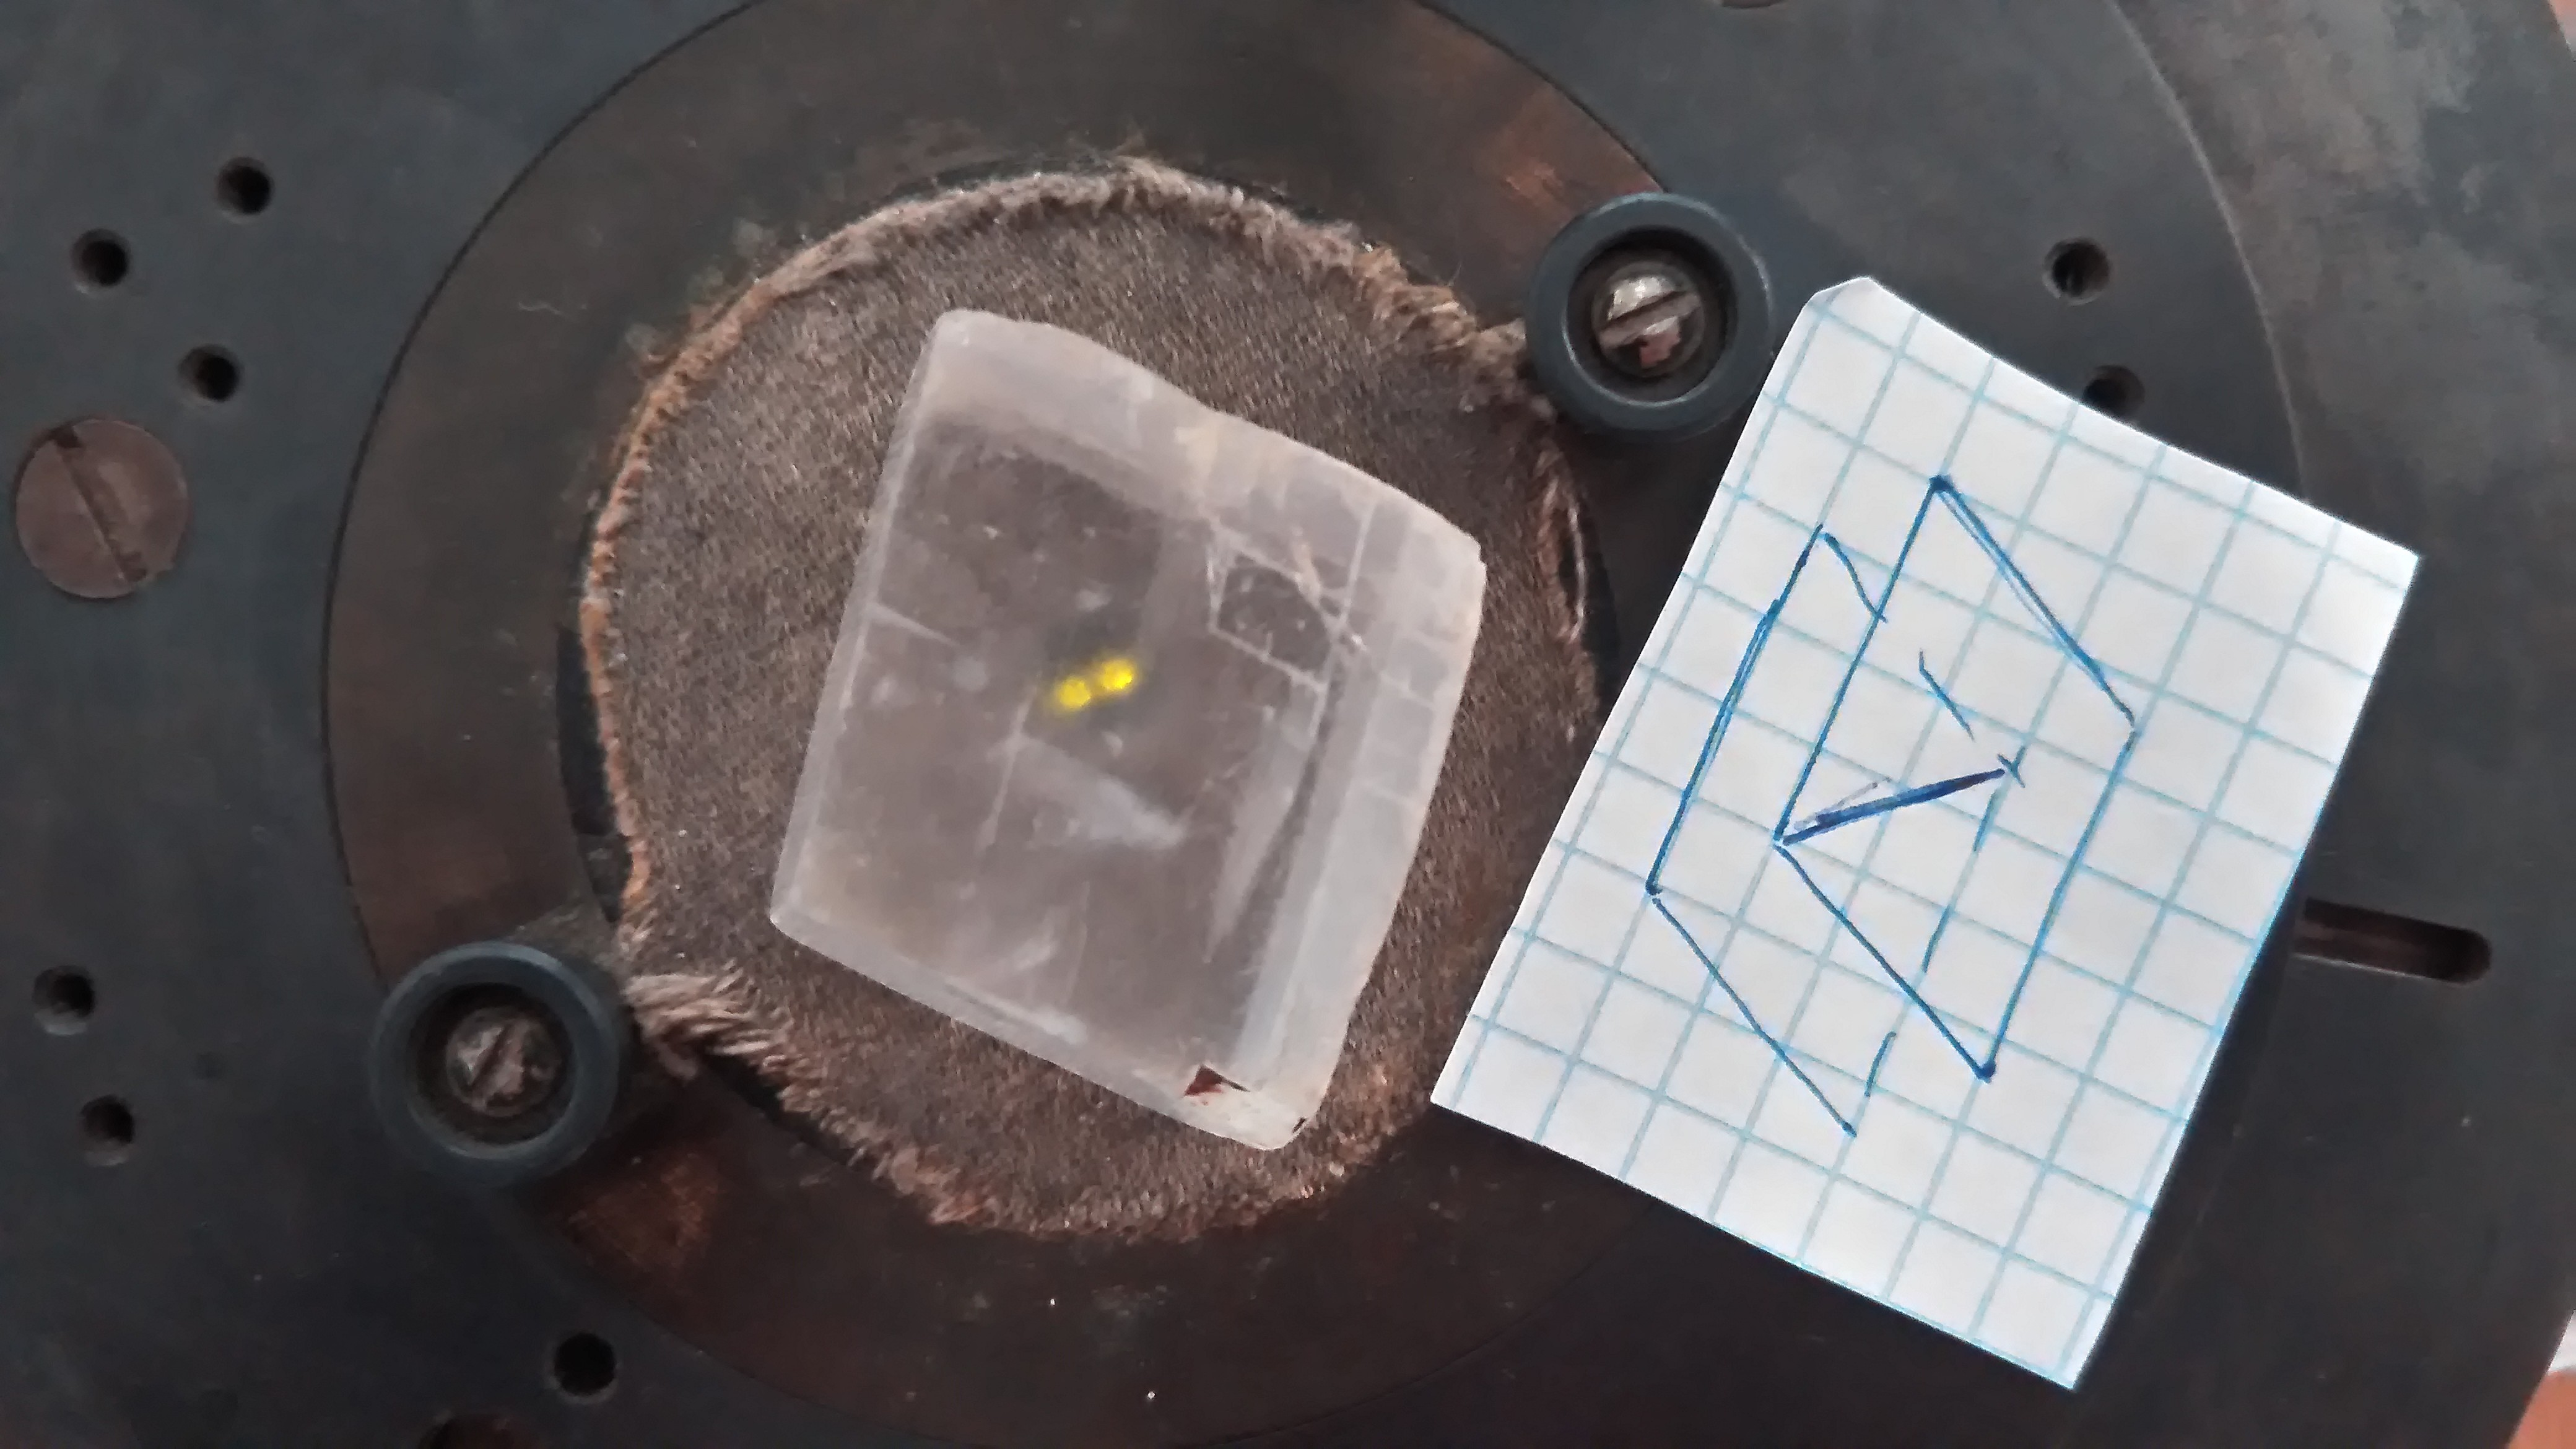
\includegraphics[width=\textwidth]{pic/rot_eo.jpg}
	\caption{Положение оптической оси}
	\label{fig:figure1}
\end{figure}

Нашли плоскость главного сечения, указали направление колебаний вектора $E$ o- и e- волн.
\begin{figure}[H]
	\centering
	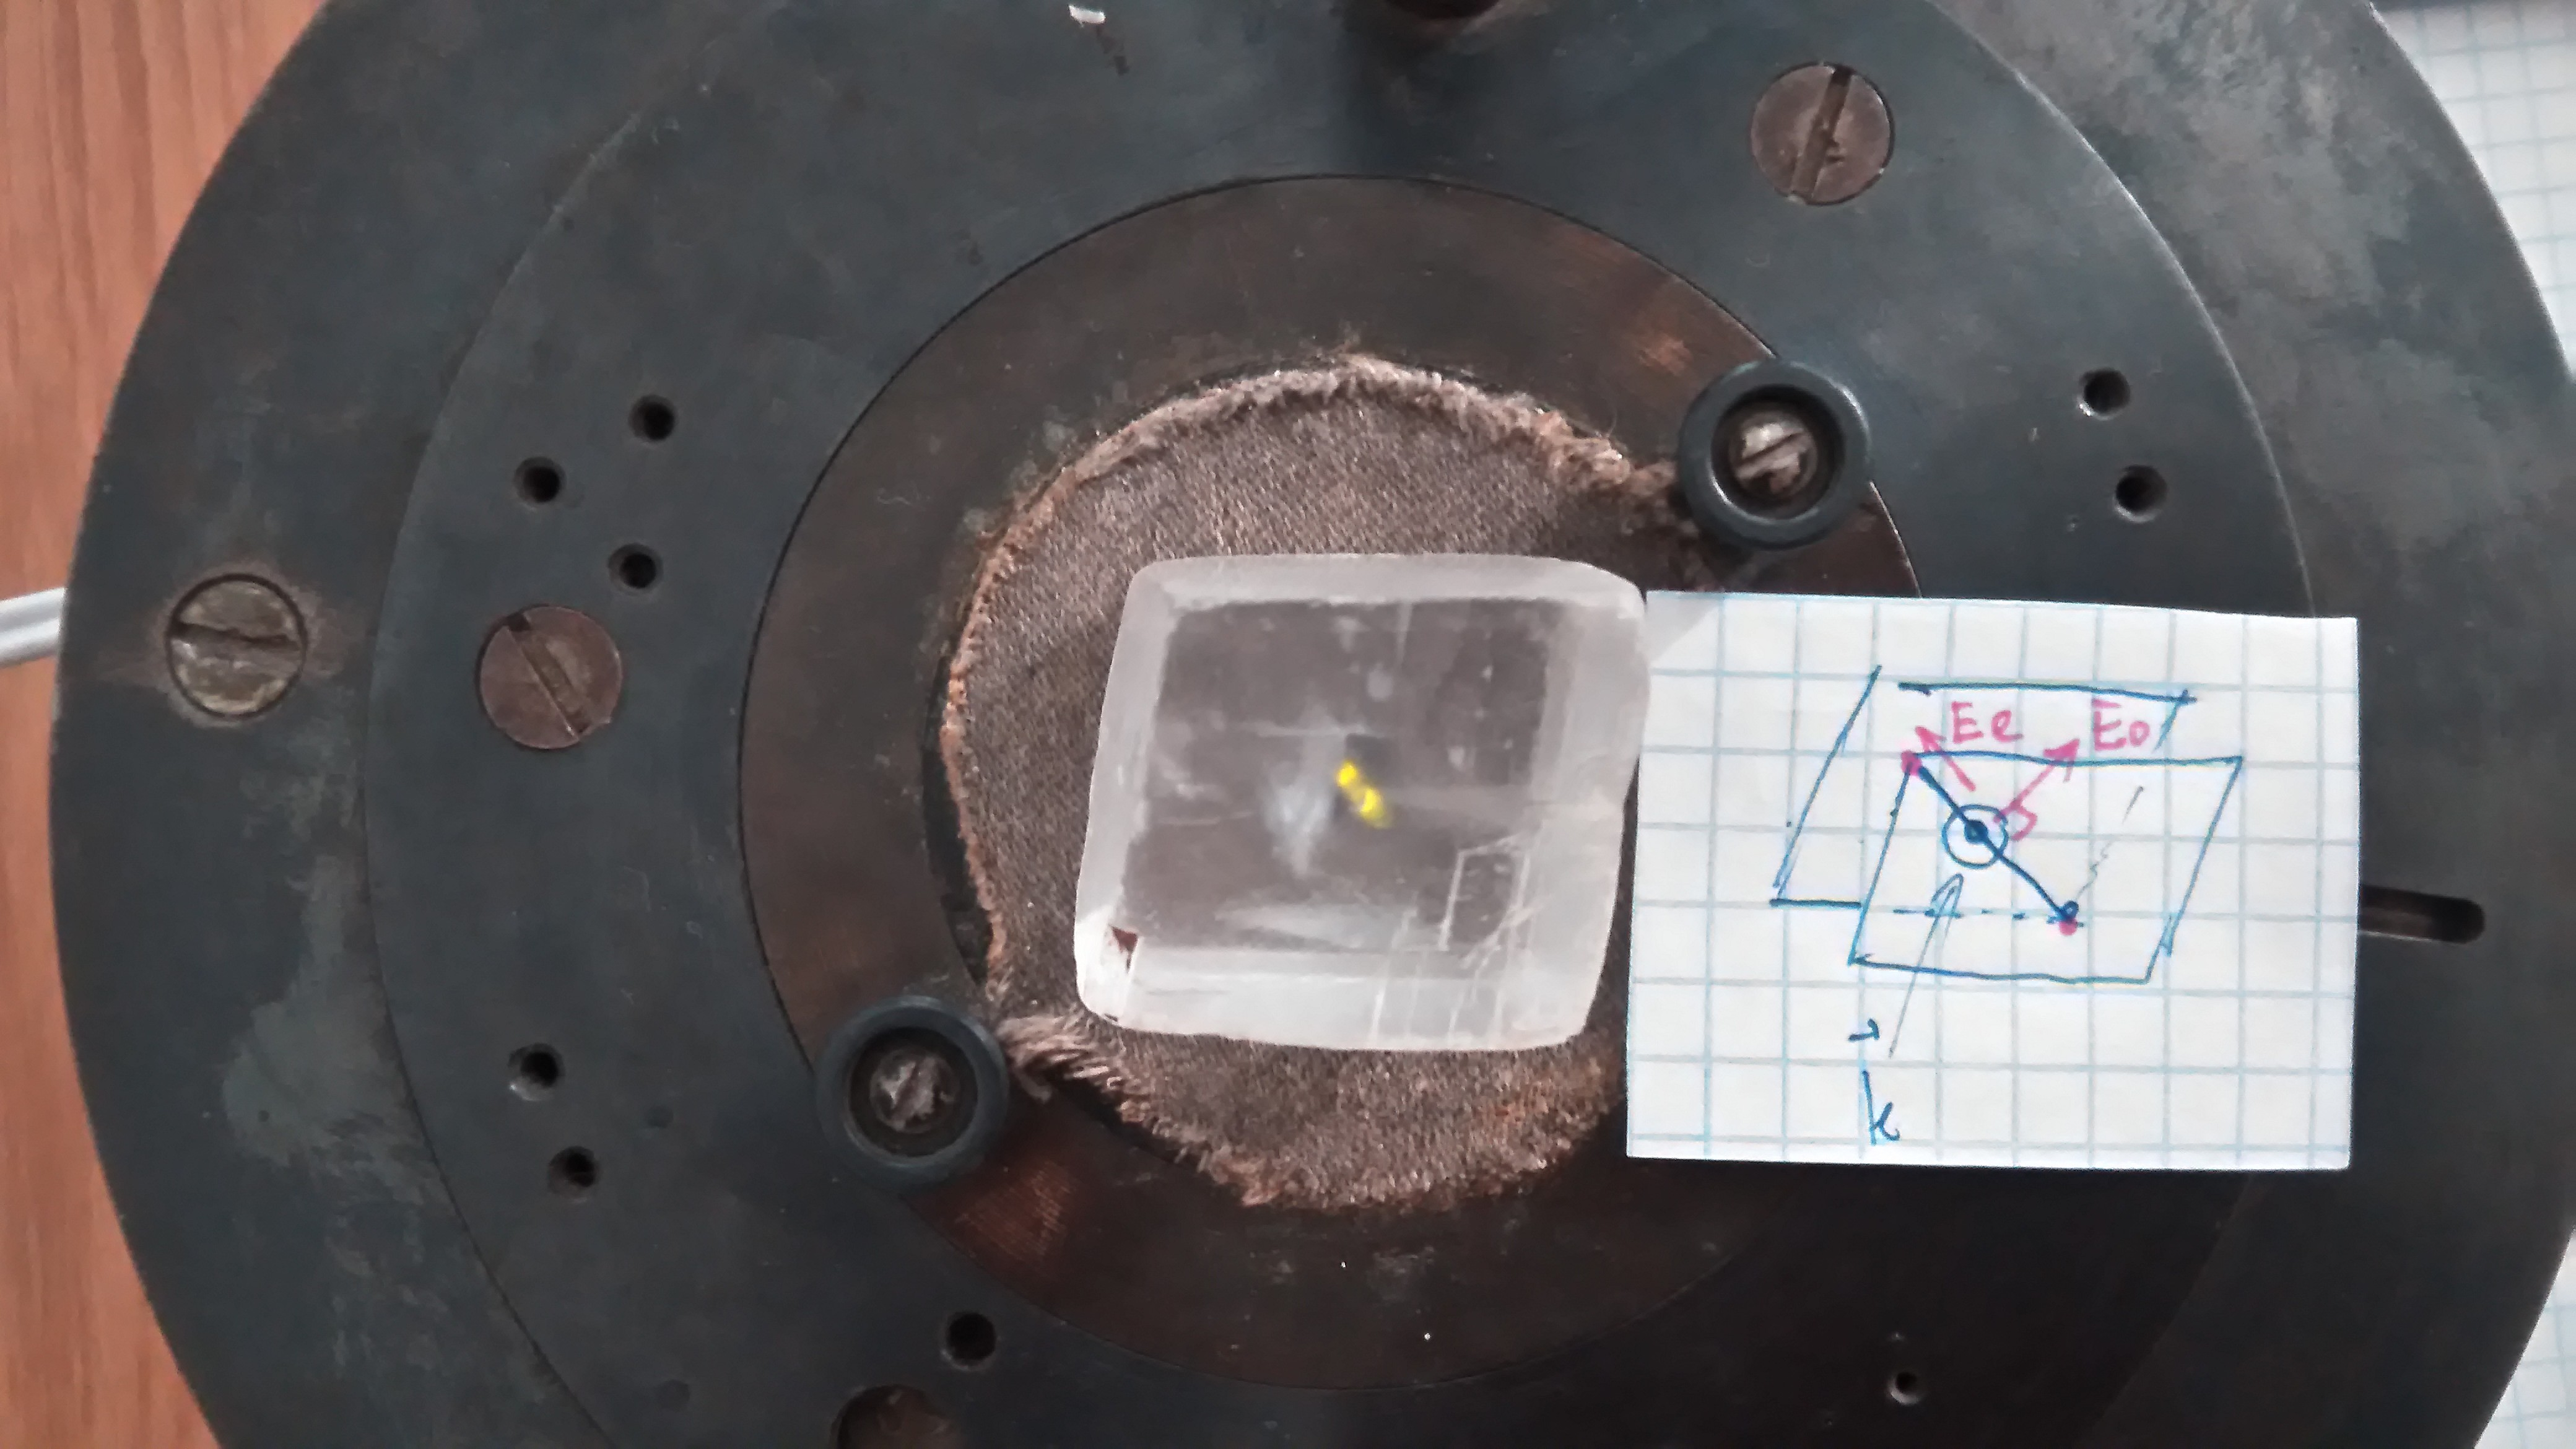
\includegraphics[width=\textwidth]{pic/eo.jpg}
	\caption{Положение плоскости главного сечения: образуется векторами $\vec{k}$ и оптической осью. Направление колебаний вектора $E$ в обыкновенной и необыкновенной волнах}
	\label{fig:figure1}
\end{figure}

\subsubsection{Полярископ}

Пронаблюдали двулучепреломление естественного света. Для этого рассмотрели светящуюся точку на кристалле. Точка, отвечающая обыкновенной волне, неподвижна при небольшом повороте кристалла и если убрать кристалл, остается на прежнем месте, а отвечающая e-волне, смещается.

\begin{figure}[H]
	\centering
	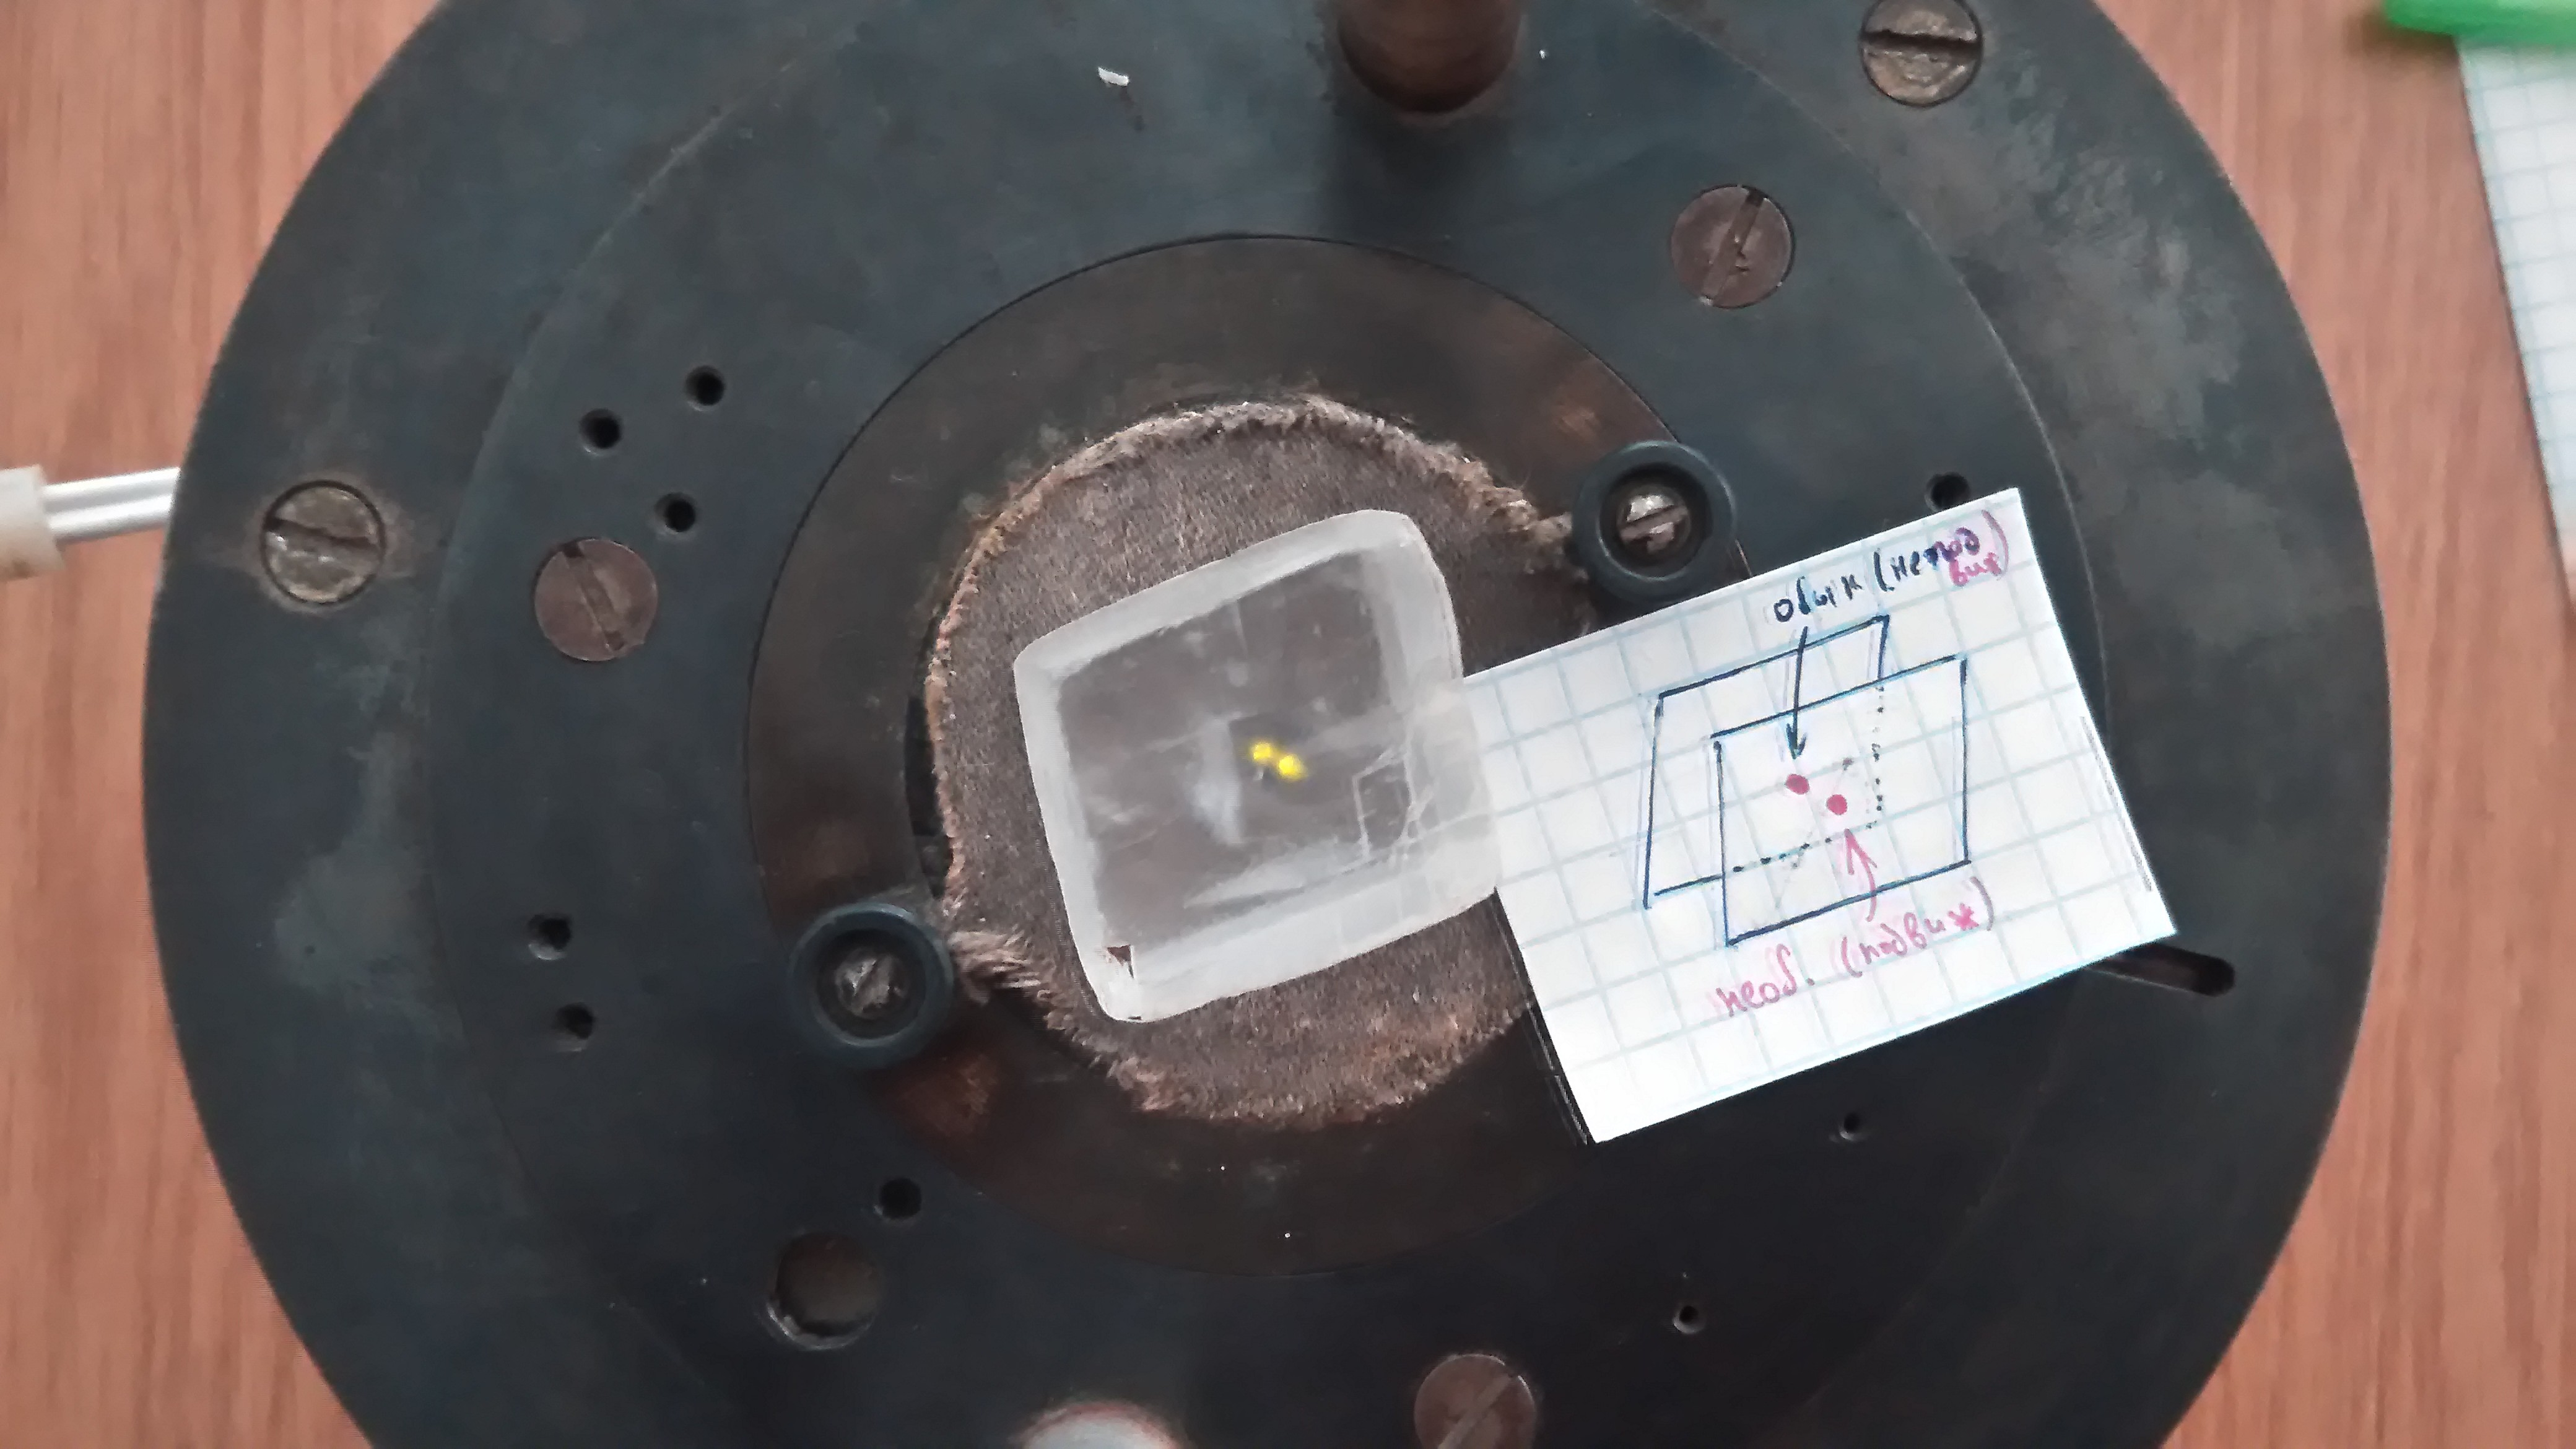
\includegraphics[width=\textwidth]{pic/dv.jpg}
	\caption{Положение точек при вращении}
	\label{fig:figure1}
\end{figure}

Вращая кристалл, получили четыре относительных положения обеих точек и положений плоскости главного сечения (относительно друг друга остаются неподвижными)

Сделали вывод, что изображение необыкновенной точки <<ближе к глазу>>

Наблюдая за кристаллом через вращаемый анализатор, заметили чередование максимума яркости одной точки и минимума другой. Смена происходит через каждые $\pi\over2$, это обосновывается перпендикулярной поляризацией e- и o- волн.
%%%%%%%%%%%%%%%%%%%%%%%%%%%%%%%%%%%%%%%%%%%%%%%%%%%%%%%%%%%%%%%%%%%%%%
\section{Часть 2}
\subsection{Поляризация световых волн при отражении и преломлении}
Энергитический коэффициент отражения плоской световой волны по определению равен
\begin{equation}
	\rho=\frac{P_1}{P}=\frac{\bar{E_1}^2}{\bar{E}^2}
\end{equation}
Здесь $P_1$ и $P$, $\bar{E_1}^2$ и $\bar{E}^2$ - соответственно потоки энергии и средние по времени квадраты напряженности электрического поля в отраженной и падающей волне.

Из формулы Френеля следует, что коэффициент отражения $\rho$ от плоской границы двух диэлектриков зависит от направления вектора $\vec{E}$ в падающей волне. Так, если вектор $\vec{E}$ перпендикулярен к плоскости падения, то 
\begin{equation}
\label{eq:2.1}
	\rho_{\bot}=\frac{\sin^2(\phi-\psi)}{\sin^2(\phi+\psi)},
\end{equation}
где $\phi$- угол падения, а $\psi$- угол преломления.

Если же вектор $\vec{E}$ параллелен плоскости падения, то
\begin{equation}
\label{eq:2.2}
	\rho_{\|}=\frac{\tg^2(\phi-\psi)}{\tg^2(\phi-\psi)}
\end{equation}

Из (\ref{eq:2.1}) и (\ref{eq:2.2}) видно, что:

1. При любом $\phi$ $\rho_{\bot}>\rho_{\|}$

2. При $\phi+\psi=\frac{\pi}{2} \label{eq:2.3} \, (\ref{eq:2.3})$
$\rho_{\bot}\neq0$ при $\rho_{\|}$.

Это означает, что в  отраженном свете всегда преобладает $E_{\bot}$.
При отражении под углом Брюстера, удовлетворяющим условию (\ref{eq:2.3})
отраженный свет полностью линейно поляризован. При этом преломленный свет оказывается частично поляризованным.

Угол отражения, удовлетворяющий соотношению (\ref{eq:2.3}), называют углом поной поляризации или углом  $\phi_{\text{Б}}$ по имени шот­ландского ученого Давида Брюстера, открывшего в 1812 году полную
поляризацию при отражении. Из закона преломления
\begin{equation}
	\frac{\sin{\phi}}{\sin{\psi}}=n
\end{equation}
и условия (\ref{eq:2.3}) следует:
\begin{equation}
	\tg\phi_{\text{Б}}=n
\end{equation}
В качестве числовой характеристики частично поляризованного света
используется понятие степени поляризации. Так, степень поляризации
отраженного света по определению равна
\begin{equation}
 	\Delta=\frac{I_{\bot}-I_{\|}}{I_{\bot}+I_{\|}}
% 	\frac{\bar{E_{\bot}^2-\bar{E^2_{\|}}{\bar{E_{\bot}^2+\bar{E^2_{\|}}}
\end{equation}
Аналогично определяется степень поляризации преломленного света
и света, прошедшего через прозрачную плоскопараллельнуго пластинку.

Прохождение света через пластинку эквивалентно двум последо­
вательным преломлениям на ее первой и второй границе с воздухом.
При каждом преломлении степень поляризации возрастает но несколь­
ко процентов (порядка $8\%$ при h= 1,52). Пропустив свет через
стопу из достаточно большого числа ( $N\approx20$) тонких пластин,
можно получить степень поляризации близкую к единице.

Таким образом, прозрачное стеклянное зеркало, зеркало из
черного стекла и стопу стеклянных пластин можно использовать в
качестве поляризатора или анализатора.


%%%%%%%%%%%%%%%%%%%%%%%%%%%%%%%%%%%%%%%%%%%%%%%%%%%%%%%%%%%%%%%%%%%%%%
\section{Часть 3}
\subsection{Интерференция поляризованного света в параллельных лучах.
Фазовые пластинки $\lambda/2$ и $\lambda/4$ и образцы для исследования. Вращение плоскости колебаний в кристаллах кварца. Опыты с удвоителем Норренберга}


Пусть линейно поляризованный свет, прошедший через узкопо­
лосный фильтр $\text{Ф}$ и поляризатор $\text{П}$ , падает на двупрелом-
ляющцую пластинку толщины d нормально к ее большим граням в
положительном направлении оси $Z$ (рис. ). Пусть, кроме того,
большие грани пластинки параллельны оптической оси $X$ , обра­
зующей углы $\alpha$ и $\beta$ с направлениями колебаний вектора $\vec{E}$
на выходе поляризатора П анализатора А соответственно
(рис.6 ). Электрическое поле $\vec{E}$ в падающем на пластинку параллель­
ном пучке можно приближенно описать уравнением плоской бегущей
волны 
\begin{equation}
	\vec{E}(t)=\vec{E}\cos(\omega t-kz)
\end{equation}
На входной грани $Z=О$ поле $\vec{E}\cos(\omega t)$ возбуждает
в пластинке два взаимно перпендикулярных колебания $\vec{E_y}$
(обыкновенная волна) и $\vec{E_x}$ (необыкновенная волна) с амплитудами $E\sin\alpha$ и $E\cos\alpha$ и разными скоростями
распространения вдоль оси Z
\begin{gather}
	V_z^{\text{об}}=V_o=\frac{c}{n_0} \\
	V_z^{\text{необ}}=V_e=\frac{c}{n_e}
\end{gather}

Здесь $n_0$ и $n_e$ -- главные показатели преломнелия обыкновенной и необыкновенной волны.

На выходе из пластинки получаются взаимоперпендикулярные колебания
\begin{gather}
	E_y=E\sin\alpha\cos(\omega t -k_yd) \\
	E_z=E\cos\alpha\cos(\omega t -k_zd),
\end{gather}
где
\begin{gather}
	k_y=\frac{\omega}{V_0}=\frac{\omega}{c}\cdot n_0=kn_0, \,
	k_x=\frac{\omega}{V_e}=\frac{\omega}{c}\cdot n_e=kn_e
\end{gather}
Эти колебания сдвинуты по фазе на величину
\begin{equation}
	\delta=(k_x-k_y)d=k(n_e-n_0)d=\frac{2\pi}{\lambda}\Delta nd,
\end{equation}
зависящую от длины волны $\lambda$ и свойств пластинки.

Разность главных показателей преломления $\Delta n=n_e-n_0$
называют величиной двупреломления или просто <<двупреломлением>>.
На вход анализатора А поступает суперпозиция двух векторных
взаимно перпендикулярных колебаний с неравными амплитудами
$E\sin\alpha$ и $E\cos\alpha$ и постоянным сдвигом фаз $\delta$, т.е. эллиптически поляризованное колебание, которое
в специальных случаях может переходить в поляризованное по кру­гу 
(при $\alpha=\pm\frac{\pi}{4}$ и $\delta=\pm\frac{\pi}{2}$. При эллиптической
поляризации конец вектора Е движется (в фиксированной плоскости
XY)ио эллипсу, ориентация которого зависит от амплитуд
$E\sin\alpha$, $E\cos\alpha$ и разности фаз $\delta$ . Из-за
зависимости $\delta(\lambda)$ положение эллипса поляризации изменяется
с изменением длины волны $\lambda$.

Анализатор А, расположенный на расстоянии $Z-d$ от
пластинки, пропускает а глаз наблюдателя сумму двух параллельных
колебаний 
\begin{gather}
	E=E\cos\alpha\cos\beta\cos\left[\omega t -k_xd-k(z-d) \right]+\\
	+E\sin\alpha\sin\beta\cos\left[\omega t -k_yd-k(z-d) \right]
\end{gather}
с приобретенным в пластинке сдвигом фаз $\delta$. Тем самым создает­
ся возможность наблюдать интерференцию в параллельном поляризо­
ванном свете. Для описания интерференционной картины необходимо
знать интенсивность света I на выходе анализатора, которая с
точностью до постоянного размерного множителя равна квадрату ам­
плитуды Е ($I\approx E^2$). Чтобы найти и получить для I выражение
удобное для интерпретации, - обозначим $E\cos\alpha\cos\beta=a_1$,
$E\sin\alpha\sin\beta=a_2$  и воспользуемся известной формулой
для квадрата амплитуды суммарного колебания:
\begin{equation}
	E^2=a_1^2+a_2^2+2a_1a_2\cos\delta=(a_1+a_2)^2-4a_1a_2\sin^2\frac{\delta}{2}
\end{equation}
После несложных тригонометрических преобразований, получаем
\begin{equation}
	\label{eq:1}
	I=I\left[\cos^2(\beta-\alpha)-\sin2\alpha\sin2\beta\sin^2\frac{\delta}{2} \right]
\end{equation}
Формула (\ref{eq:1}) описывает все возможные случаи прохождения параллельных линейно поляризованных лучей через пластинку, параллельную
оптической оси, и анализатор. Особый интерес представляет слу­чай наблюдения в скрещенных и в параллельных николях.

При скрещенных николях $\beta-\alpha=\frac{\pi}{2}$ и
\begin{equation}
	I_{\bot}=I\sin^22\alpha \sin^2\frac{\delta}{2}
\end{equation}

При параллельных николях $\beta-\alpha=0$ и 
\begin{equation}
	I_{\|}=I\left(1-\sin^22\alpha \sin^2\frac{\delta}{2}\right)
\end{equation}

Следовательно
\begin{equation}
\label{eq:2}
I_{\bot}+I_{\|}=I	
\end{equation}
Соотношения (\ref{eq:2}) справедливы для каждой спектральной компоненты в случае падающего на устройство белого света. Суммируя равенства (\ref{eq:2})
для компонент белого света получим
\begin{equation}
	\sum_{\lambda} I_{\bot}+\sum_{\lambda} I_{\|}=\sum_{\lambda} I
\end{equation}
Как видно из формулы (\ref{eq:1}) интенсивность в интерференционной
картине зависит от величины $\delta$. Рассматривая двупреломляющую
пластинку через анализатор, глаз будет видеть ее светлой, темной
или в разных местах различно окрашенной в зависимости от эначе-
ния и распределения сдвига фаз $\delta$ по поверхности пластины.
Сам сдвиг фаз $\delta$ , как видно из (), зависит от порядка интерференции
 $m=\frac{\Delta nd}{\lambda}$. При низких порядках интерферен­ции наблюдаются цветные интерференционные окраски, появление ко­торых следует из структуры формулы (\ref{eq:1}), в которой первое слага­емое $\cos^2(\beta-\alpha)$ постоянно для всех цветов, а второе -
содержащее множитель $\sin^2\frac{\delta}{2}$, зависит от $\lambda$. Наиболее сочные интерференционные окраски наблюдаются в скрещенных
николях, когда $\cos^2(\beta-\alpha)=0$ , а амплитуды $E\sin\alpha$
и $E\cos\alpha$ одинаковы. Положение пластинки, при котором
$E\cos\alpha=E\sin\alpha$ и $\alpha=\pm\frac{\pi}{4}$ называется <<диаго­
нальным>>, оно особенно благоприятно для наблюдения интерференци­
онных окрасок при освещении белым светом.

Для изменения характера поляризации и анализа поляризован­
ного света применяют фазовые пластинки в половину и в четверть
длины волны. Это двупреломляющие пластинки, параллельные опти­
ческой оси, на выходе из которых сдвиг фаз между обыкновенной и
необыкновенной волной равен $\pm\pi$ или $\pm\frac{pi}{2}$, соответствен­
но. Толщины полуволновых и четверть-волновых пластинок вычисляются из условия $\Delta d=\frac{\lambda}{2}$ и $\Delta nd=\frac{\lambda}{4}$.Фазовые
пластинки чаще всего изготовляют из таких природных кристаллов,
как исландский шпат ($CaCO_3$), кварц ($SiO_2$) и слюда.

При работе с образцами из кварца следует иметь в виду, что
кварц, наряду с двойным преломлением, обладает еще одним удивительным свойством совсем иной природы, а именно - способностью
вращать плоскость колебаний линейно поляризованного света. Эта
способность называется оптической активностью и обусловлена особым, винтовым расположением молекул $SiO_2$ в кристаллической решетке кварца. Вращение плоскости колебаний наиболее сильно
выражено именно тогда, когда двойное преломление отсутствует, т.
е. при распространении света в кристалле по направлению оптичес­
кой оси.
В природе встречаются две модификации кристаллов кварца -
правей и левая. В правых и левых кристаллах плоскости колебаний
поворачиваются в противоположных направлениях. Если для наблю­дателя, смотрящего навстречу световому лучу, плоскость колебаний
на выходе из кварца повернута по часовой стрелке, то такой кварц
называется правовращающим или правым. Для того, чтобы избежать
неоднозначности при экспериментальном определении направления
вращения в кварце, толщина исследуемого образца должна быть дос­таточно мала (не более одного миллиметра).
Угол поворота плоскости колебаний в кварце пропорционален
толщине образца d и равен $\alpha=\alpha_1d$, где $\alpha_1$-удельное вращение, измеряемое в град/мм. Величина $\alpha_1$ сильно зависит от длины волны и быстро увеличивается при переходе от красеого света к фиолетовому. 
Зависимость $\alpha_1(\lambda)$ называет­ся дисперсией вращения плоскости колебаний или дисперсией оптической активности.
Если на вход кварцевой пластинки поступает линейно поляризованный белый свет,то на ее выходе плоскости колебаний различных спектральных компонент поля $\vec{E}(\lambda)$ развернуты в "цветовой
веер", от красного цвета к фиолетовому.
\subsection{Бикварц}
Бикварц состоит из двух одинаковых полукруглых пластинок
из левого и правого кварца, склеенных по диаметральному сечению.
Толщина обеих половинок одинакова и равна 3,75 мм. При такой
толщине плоскости колебаний фиолетового света на выходе из би­кварца повернуты в противоположных направлениях на 180°, а плос­кости колебаний наиболее ярких в спектре зеленовато-жеелтых лучей - на 90°. Поэтому, в параллельных николях зеленовато-желтый
свет будет полностью погашен, я фиолетовый - полностью пропущен,
и при точной установке николей обе половинки бикварца будут окра­
шены в характерный серовато-фиолетовый оттенок.
При скрещенных николях окраска сменится на дополнительную
зеленовато-желтого оттенка. Малейшее отклонение одного из николей от параллельной или скрещенной установки вызывает резкое раз­личие в окраске обеих половинок бикварца. Поэтому бикварц позво­ляет установить николи в параллельное или скрещенное положение с
более высокой точностью, чем при обычной установке их на темноту.
\subsection{Практическая часть}
\subsubsection{Определение типа пластинок}
Поставив анализатор на темноту, наблюдали изменение интенсивности при вращении пластинок. 
Таким образом было обнаружено, что в нашем распоряжении одна кварцевая пластинка, две четверть-волновых и одна полуволновая.




%%%%%%%%%%%%%%%%%%%%%%%%%%%%%%%%%%%%%%%%%%%%%%%%%%%%%%%%%%%%%%%%%%%%%%%%%%%%%%%
\newpage
\section{Заключение}

\end{document}